\chapter{Developing MOOSE Applications with ICE}
\label{sec:devMoose}

\section{Introduction}\label{introduction}

This article is designed to walk MOOSE developers through a typical
workflow for developing MOOSE-based applications in ICE. Since ICE is
built on top of the Eclipse platform, a large variety of sophisticated
software development tools and technologies for developing scientific
software can be integrated into the ICE platform. Version control, code
editing, code completion, code building, and code generation are just a
few of the various technologies now available to MOOSE-based application
developers using ICE. Additionally, after developing your custom MOOSE
application, the usual MOOSELauncher and MOOSEModel Items and the ICE
Visualization perspective are still at your disposal for constructing
input files, launching jobs, and visualizing results.

\section{Cloning MOOSE}\label{cloning-moose}

To clone MOOSE, simply switch to the Git Perspective in the top right
corner of ICE. You will be presented with the following view.

\begin{figure}[htbp]
\centering
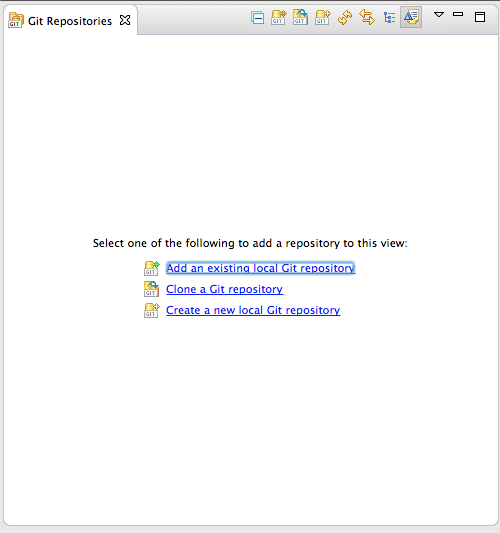
\includegraphics[width=\textwidth]{figures/GitView.png}
\caption{A view of the ICE Git Perspective.}
\end{figure}

Now click the 'Clone a Git Repository' button in the toolbar of the 'Git
Repository' view (or the hyperlink in the middle of the view if you have
not repositories). You will be presented with the following wizard.

\begin{figure}[htbp]
\centering
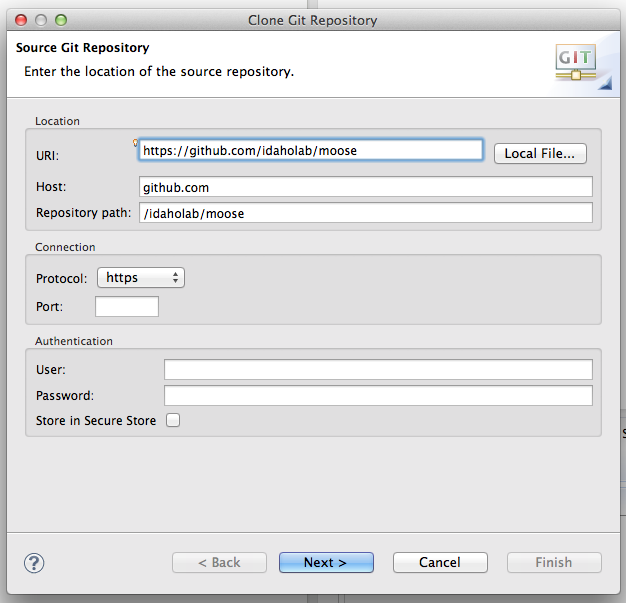
\includegraphics[width=\textwidth]{figures/Clone_wizard.png}
\caption{The first page of the Clone Repository Wizard requesting information about the remote Git repository URL.}
\end{figure}
\begin{figure}[htbp]
\centering
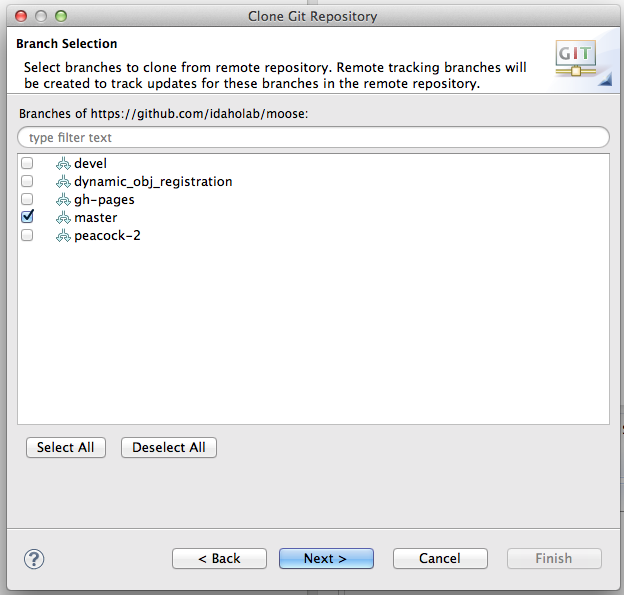
\includegraphics[width=\textwidth]{figures/Clone_wizard2.png}
\caption{The second page of the Clone Repository Wizard requesting information about which branches to pull down.}
\end{figure}
\begin{figure}[htbp]
\centering
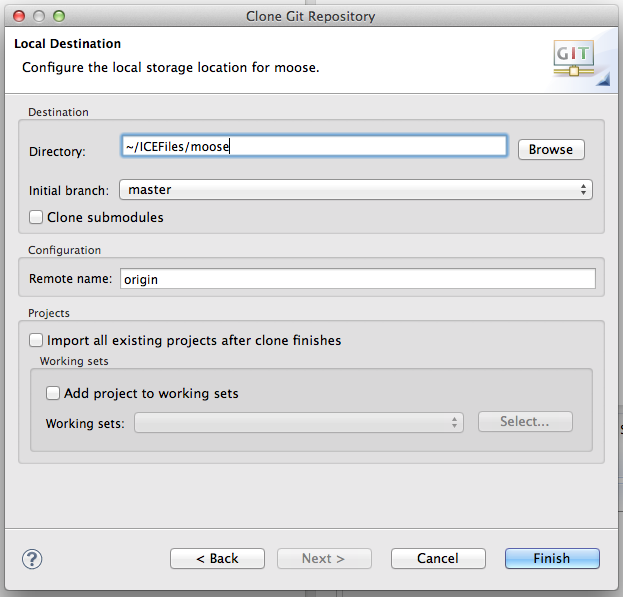
\includegraphics[width=\textwidth]{figures/Clone_wizard3.png}
\caption{The final page of the Clone Repository Wizard requesting information about the local location of the repository.}
\end{figure}

Enter \url{https://github.com/idaholab/moose} into the URI entry and
select next. This will present you with the branch selection wizard
page. Select which branches you'd like to import in this clone and click
Next. The last page will let you specify the clone location on your
local filesystem. If you'd like this to be in your local ICE workspace
entry /home/username/ICEFiles in the entry and click Finish.

To import MOOSE into your ICE Project Explorer, simply right click the
created moose repository in the Git Repository view and select 'Import
Projects'. On the first wizard page, select 'Import as New Project' and
click finish. This will present you with the ICE New Project wizard. In
this wizard, open the C/C++ tree node and select 'Makefile project with
Existing Code'. Provide a valid project name and toolchain and click
finish. You should see MOOSE in your Project Explorer.

\begin{figure}[htbp]
\centering
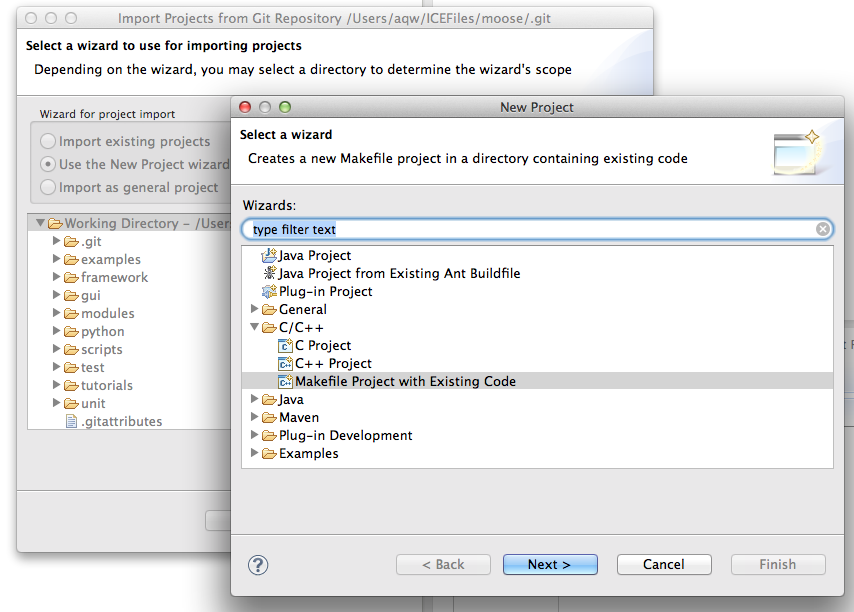
\includegraphics[width=\textwidth]{figures/Import_git_proj.png}
\caption{The import projects wizard for the ICE Git repositories view. }
\end{figure}

\section{Building MOOSE}\label{building-moose}

To build MOOSE/Libmesh within ICE, open the Make Target view by going to
Window \textgreater{} Show View \textgreater{} Other and search and
select Make Target. With MOOSE imported into your Project Explorer, you
should see the MOOSE project in the Make Target view. Right click on
that project and select New. A dialog will pop up prompting you for the
Make Target name, target name, and build command. Set the name as 'Build
Libmesh', uncheck 'Same as target name' and leave the Make target blank,
uncheck 'Use builder settings' and set the command as 'sh
scripts/update\_and\_rebuild\_libmesh.sh', then click 'Ok'. Now you
should see a 'Build Libmesh' target, which upon double-clicking will
execute the update\_and\_rebuild\_libmesh.sh script with the output
streaming in the Console view.

Once that is done, you can create another Make Target in the same
manner, this time setting the target as all, but setting the build
command (assuming you have CMake installed on your system) as 'cmake -E
chdir framework make' (feel free to add -j N to this command, where N is
the number of make threads). If you do not have CMake installed, you can
right click on the MOOSE project in the Project Explorer and select
Properties. In this Properties dialog, select C/C++ Build and append to
the Build directory entry 'framework'. Now, double-clicking this make
target will execute the MOOSE build, and you should see the output
streaming in the Console.

\section{Forking the Stork}\label{forking-the-stork}

The internal MOOSE development team provides another GitHub repository
called stork at \url{https://github.com/idaholab/stork} that represents
the base structure needed to create a new MOOSE application. So 'Forking
the Stork' implies forking this repository, changing its name to
whatever you've decided to call your MOOSE application, and cloning that
locally to begin work. The MOOSE team calls this 'Forking the Stork' and
provides a link to the repository at mooseframework.org/create-an-app.

ICE now provides this functionality in an easy-to-use toolbar button
using the tools provided by the Eclipse EGit plugins. To 'Fork the
Stork' in ICE, simply click the 'MOOSE Fork the Stork' button in the
toolbar.

\begin{figure}[htbp]
\centering
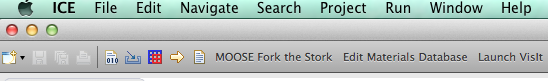
\includegraphics[width=\textwidth]{figures/Fork_button.png}
\caption{The ICE Fork the Stork button in the toolbar. }
\end{figure}
\begin{figure}[htbp]
\centering
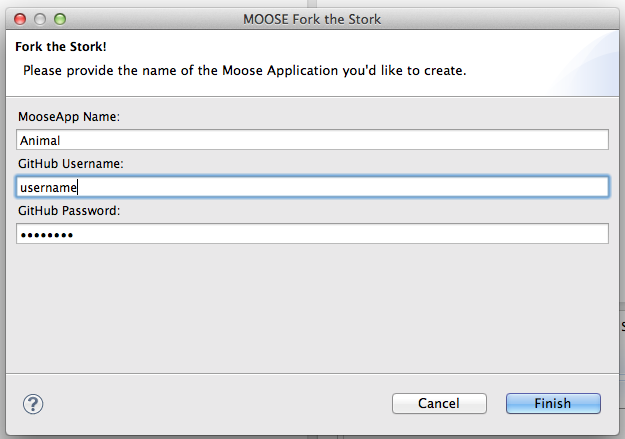
\includegraphics[width=\textwidth]{figures/Fork_dialog.png}
\caption{The Fork the Stork Wizard for entering your new MOOSE application name and your GitHub credentials.}
\end{figure}

This will present a new dialog asking for the name of your new MOOSE
application, as well as your GitHub username and password. Upon
providing this information and clicking 'Ok', ICE will fork the
\url{https://github.com/idaholab/stork} repository for you, rename it to
your provided application name, clone it to \textasciitilde{}/ICEFiles,
and import it into ICE as a new C++ project in the C/C++ perspective's
Project Explorer view.

Additionally, the import generates a fully configured Make Target in the
Make Target view, and sets up the C++ Indexer to point to your ICE MOOSE
project's include files. This is essential for providing code completion
and MOOSE code search while your developing your MOOSE application. To
look at a MOOSE class that you've referenced in one of your
application's source files, simply click the class name or the header
file and click F3. ICE will take you directly to the declaration for
that MOOSE class so that you can peruse and look up its method
definitions.

\begin{figure}[htbp]
\centering
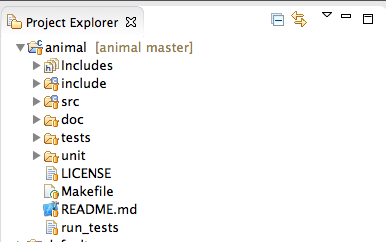
\includegraphics[width=\textwidth]{figures/New_app.png}
\caption{ICE creates the newly forked MOOSE application as a C/C++ project in the Project Explorer.}
\end{figure}
\begin{figure}[htbp]
\centering
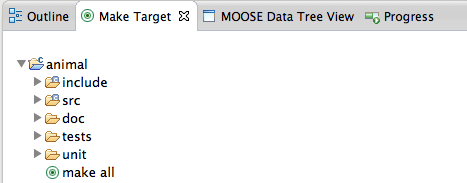
\includegraphics[width=\textwidth]{figures/Make_target.png}
\caption{ICE adds a new Make Target to the Make Targets View for building your new application.}
\end{figure}

\newpage

\section{Adding a New Kernel}\label{adding-a-new-kernel}

Once you've cloned and built MOOSE, and Forked the Stork to produce a
new MOOSE application ready for development, you can easily create
custom Kernels with ICE. To create a new Kernel, right click on your new
MOOSE-based application project and select New \textgreater{} MOOSE
Object \textgreater{} Kernel.

\begin{figure}[htbp]
\centering
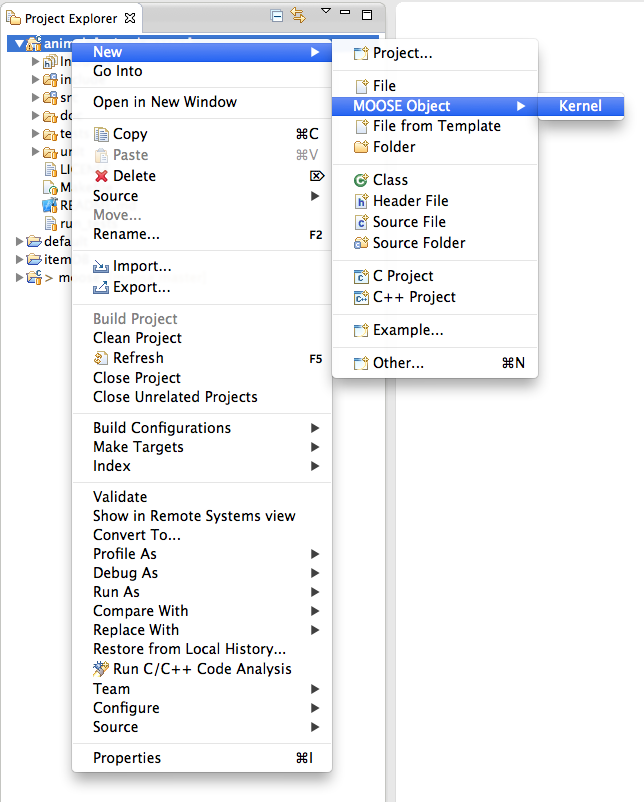
\includegraphics[width=\textwidth]{figures/New_kernel.png}
\caption{Creating a new Kernel in ICE is easy, just right click on your project and select New - MOOSE Object - Kernel.}
\end{figure}

This action will display an input prompt asking for the name of your new
Kernel subclass. Simply enter the name and push 'Ok'. Then ICE will
automatically generate a new include and source file in include/kernel
and source/kernel, respectively. The new files are the stubbed out, base
implementation of a subclassed Kernel that you can then add to and
modify.

\begin{figure}[htbp]
\centering
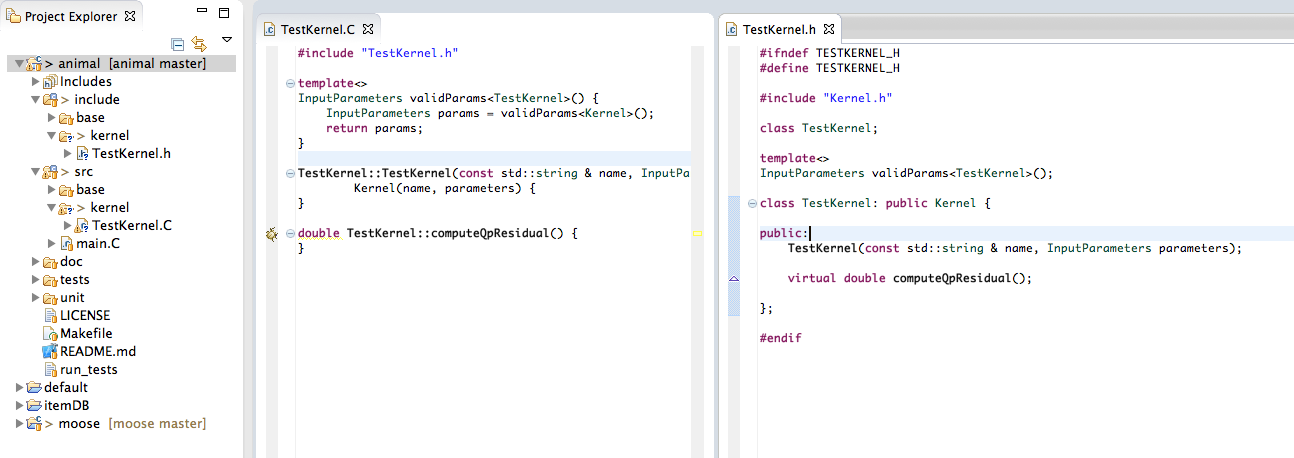
\includegraphics[width=\textwidth]{figures/Kernel_source.png}
\caption{The created source code for the Add Kernel context menu action. }
\end{figure}

\section{Building your MOOSE App}\label{building-your-moose-app}

Building your MOOSE application is simple because the 'Fork the Stork'
action produced a Make Target for you. Simply double-click that make
target and you application will build, producing the application
executable.

\section{Pushing Changes Back to
GitHub}\label{pushing-changes-back-to-github}

To push changes to the remote GitHub repository at
\url{https://github.com/username/animal}, switch back to the Git
perspective and click your applications git repository in the Git
Repositories view. On the bottom right of the screen, you should see
another set of tabbed views, one of them being the Git Staging view.

\begin{figure}[htbp]
\centering
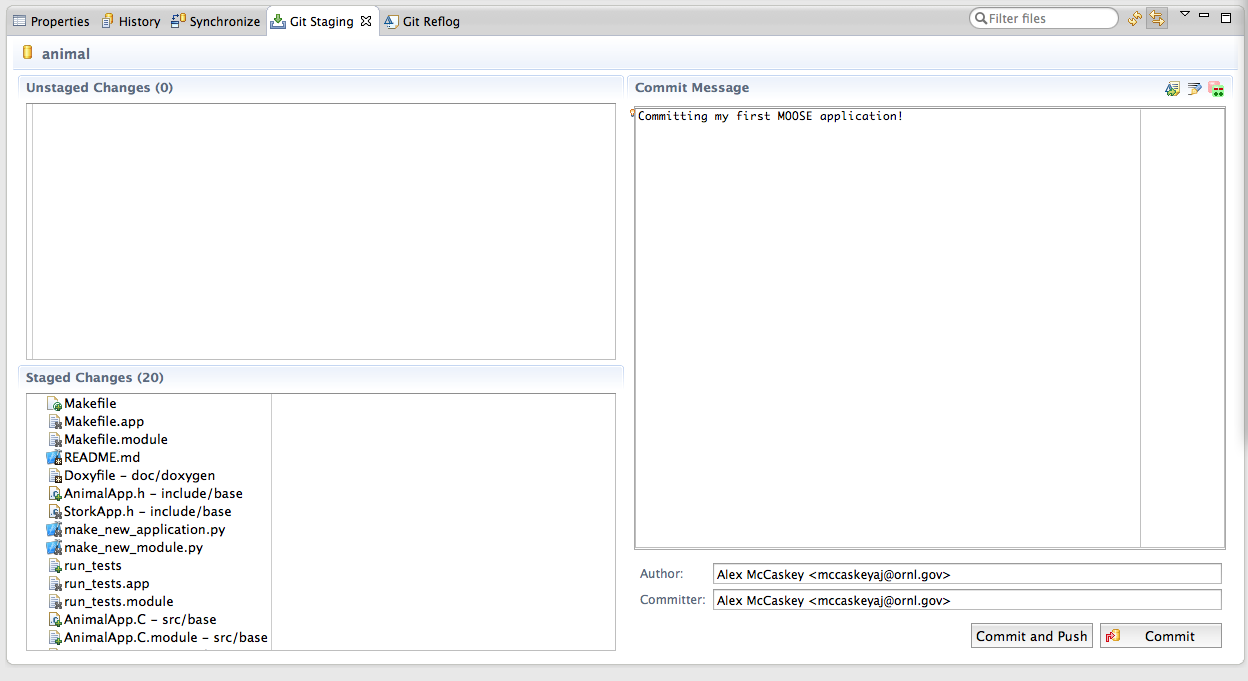
\includegraphics[width=\textwidth]{figures/Git_commit.png}
\caption{Committing your new MOOSE application is easy, just stage it in the Git Staging view of the Git Repositories Perspective.}
\end{figure}

Click the Git Staging View and drag any Unstaged Changes to the Staged
Changes section. Now provide a brief commit message and click 'Commit
and Push', enter your GitHub credentials, and watch as your files are
committed to the remote repository!

\section{Executing Built MOOSE
Application}\label{executing-built-moose-application}

Now that you've developed a new MOOSE application you need to develop
input files for it and execute it to see your desired results. This is
simple with ICE: just use the built in MOOSE Model Builder and MOOSE
Launcher Items. Detailed instructions can be found at
\href{Using MOOSE with ICE}{Using MOOSE with ICE}.
